\documentclass[xcolor=dvipsnames]{beamer}
%\documentclass[handout,xcolor=dvipsnames,pdftex,hyperref={colorlinks=false}]{beamer}
\usetheme[height=7mm]{Rochester}
\setbeamertemplate{items}[ball]
\setbeamertemplate{blocks}[rounded][shadow=true]
\usepackage{xcolor}
\usepackage{colortbl}
\usepackage{multirow}
\usepackage{amsmath,amsthm,amssymb}
\usepackage{amsfonts}
\usepackage{epsfig}
\usepackage{times}
\usepackage[T1]{fontenc}
\usepackage{inconsolata}
\usepackage{fancyvrb}
\usepackage{bbm}
\usepackage{subcaption}
\usepackage[normalem]{ulem}

\newcommand{\Plus}{\mathord{\tikz\draw[line width=0.3ex, x=1ex, y=1ex] (0.5,0) -- (0.5,1)(0,0.5) -- (1,0.5);}}


\newcommand{\lra}{\leftrightarrow}
\newcommand{\ra}{\rightarrow}
\newcommand{\la}{\leftarrow}
\newcommand{\mc}{\mathclap}

\usepackage{tikz}
\usetikzlibrary{positioning}
\usetikzlibrary{shapes,decorations,arrows,calc,arrows.meta} 
\tikzset{
	-latex,auto,node distance = 1.5cm and 1.5cm,
	semithick ,
	state/.style ={ellipse, draw, minimum width = 0.5 cm},
    old inner xsep/.estore in=\oldinnerxsep,
    old inner ysep/.estore in=\oldinnerysep,
	el/.style = {inner sep=2pt, align=left, sloped},
	point/.style = {circle, draw=black, inner sep=0.04cm,
	 fill=black,
                node contents={}},
}

% == theme & colors
\usetheme{Warsaw}  % Jens' previous
%\usepackage{helvet}
\definecolor{someblue}{rgb}{0,.1,0.8}

\title{PS 200C: Causal inference for social science}
\date{Spring 2025}
\subtitle[ ]{Causal Graphs and Causal Structural Models}
\author{Chad Hazlett}
\institute[UCLA]{UCLA\\[1ex]
  \texttt{chazlett@ucla.edu}}

\definecolor{dgreen}{rgb}{0,.6,0.8}
\newtheorem{assumption}{Assumption}
\newtheorem{arule}{Rule}
\newtheorem{iass}{Identification Assumption}
\newtheorem{ires}{Identification Result}
\newtheorem{estm}{Estimand}
\newtheorem{esti}{Estimator}
\newtheorem{question}{Question}
\newtheorem{answer}{Answer}
\newtheorem{proposition}{Proposition}
\newtheorem{corrolary}{Corrolary}

\newcommand{\bs}{\boldsymbol}
\newcommand{\mb}{\mathbf}
\newcommand{\real}{\mathbb{R}}
\renewcommand{\u}{\ensuremath{\mb{u}}}
\renewcommand{\v}{\ensuremath{\mb{v}}}
\newcommand{\U}{\ensuremath{\mb{U}}}
\newcommand{\Z}{\ensuremath{\mb{Z}}}
\newcommand{\PP}{\ensuremath{\mb{P}}}
\newcommand{\M}{\ensuremath{\mb{M}}}
\newcommand{\X}{\ensuremath{\mb{X}}}
\newcommand{\x}{\ensuremath{\mb{x}}}
\newcommand{\Y}{\ensuremath{\mb{Y}}}
\newcommand{\D}{\ensuremath{\mb{D}}}
\newcommand{\y}{\ensuremath{\mb{y}}}
\renewcommand{\b}{\ensuremath{\bs{\beta}}}
\newcommand{\e}{\ensuremath{\bs{\epsilon}}}
\newcommand{\bhat}{\ensuremath{\hat{\bs{\beta}}}}
\newcommand{\XX}{\ensuremath{\X'\X}}
\newcommand{\XXinv}{\ensuremath{\left(\XX\right)^{-1}}}
\newcommand{\hatsig}{\ensuremath{\hat{\sigma}^2}}
\newcommand{\sig}{\ensuremath{\sigma^2}}
\newcommand{\hatmat}{\ensuremath{\X \XXinv \X'}}
\newcommand{\ehat}{\ensuremath{\hat{\e}}}
\newcommand{\tr}{\text{tr}}
\newcommand{\Sig}{\ensuremath{\bs{\Sigma}}}
\newcommand{\SigInv}{\ensuremath{\bs{\Sigma^{-1}}}}
\newcommand{\W}{\ensuremath{\mb{W}}}
\newcommand\E{\mathbb{E}}

\newcommand{\indep}{{\bot\negthickspace\negthickspace\bot}}
%\newcommand{\indep}{\mbox{$\bot\!\!\!\bot$}}


\useoutertheme{infolines}
\begin{document}


\subject{Talks}
\AtBeginSection[]
{
  \begin{frame}<beamer>
    \frametitle{Outline}
    \tableofcontents[currentsection]
  \end{frame}
}



%
%\AtBeginSubsection[]
%{
%  \begin{frame}<beamer>
%    \frametitle{Outline}
%    \tableofcontents[currentsection,currentsubsection]
%  \end{frame}
%}

\begin{frame}
  \titlepage
\end{frame}

\section{Introduction}

\begin{frame}{Resources for this material}

\onslide<1-> Today we will just get our feet wet with a superficial exploration of the graphical approach. We don't want to get caught up in details. \\
\medskip
\onslide<2-> But, for more DAG material:\\
\bigskip
\begin{itemize}
\small
\item  \textit{What if} (Hernan and Robins), Chapters 6, 7.
\item  \textit{Primer} (Pearl, Glymour, Jewell), Chapters 1.4, 1.5, 2, 3.
\item  Pearl, J. (2009).  \textit{Causality} \\
\item<3-> Some online materials:\\
\begin{itemize}
\footnotesize
\item \textit{Causal Diagrams: Draw Your Assumptions Before Your Conclusions} course by Miguel Hernan on EdX
\item \textit{A Crash Course in Causality: Inferring Causal Effects from Observational Data} course by Jason Roy on Coursera.
\item Richard McElreath lecture on ``Science before statistics: causal inference''. \url{https://www.youtube.com/watch?v=KNPYUVmY3NM&t=8565s}
\end{itemize}
\end{itemize}
\end{frame}

\begin{frame}{Goals for this lecture}
\begin{itemize}
\item<2-> Introduction to structural causal models
\bigskip
\item<3-> Graph basics: 
\begin{itemize}
\item<4-> conditional independence and d-separation
\medskip
\item<5-> backdoor criterion
%\medskip
%\item<4-> Then formalize these into tools for answering questions such as: 
%\small
%\begin{itemize}
%\item<4-> How to tell if an effect is identifiable and what to condition on
%\item<5-> See how potential outcomes emerge from graphs 
%\item<6-> Start to see how \textcolor{Blue}{conditions for identification on a graph} equate to \textcolor{Blue}{statements about conditional ignorability} we rely on with potential outcomes.
\end{itemize}
\medskip
\item<6-> Use cases for DAGs, connection to CI/SOO, handling complaints
\smallskip
\item<7-> Important things revealed by DAGs
\end{itemize}
\end{frame}



%
%
%\begin{frame}{Illustration of Simpson's Paradox}
%\normalsize
%\onslide<1-> Suppose people self-select into taking a new drug. You find: \\
%\pause
%\begin{table}[]
%\begin{tabular}{lll}
%                              & \multicolumn{2}{c}{Outcome:  Recovery}                                                                  \\
%                              & Drug                                               & No Drug                                            \\ \cline{2-3} 
%\multicolumn{1}{l|}{Men}      & \multicolumn{1}{l|}{81 of 87 (93\%)}   & \multicolumn{1}{l|}{234 of 270  (87\%)} \\ \cline{2-3} 
%\multicolumn{1}{l|}{Women}    & \multicolumn{1}{l|}{192 of 263 (73\%)} & \multicolumn{1}{l|}{55 of 80  (69\%)}   \\ \cline{2-3} 
%\multicolumn{1}{l|}{Combined} & \multicolumn{1}{l|}{273 of 350 (78\%)}  & \multicolumn{1}{l|}{289 of 350 (83\%)} \\ \cline{2-3} 
%\end{tabular}
%\end{table}
%
%\begin{itemize}
%\item<3-> Among men, those on the drug did better (93\% vs. 87\%)
%\item<4-> Among women, those on the drug did better (73\% vs. 69\%)
%\item<5-> But if you looked to combined data, you'd think people did better without the drug (78\% vs. 83\%)
%\end{itemize}
%\onslide<6-> Conclusion: give the drug to men and women, but only if you know their gender?
%\end{frame}
%
%
%\begin{frame}{Illustration of Simpson's Paradox}
%\begin{table}[]
%\begin{tabular}{lll}
%                              & \multicolumn{2}{c}{Outcome:  Recovery}                                                                  \\
%                              & Drug                                               & No Drug                                            \\ \cline{2-3} 
%\multicolumn{1}{l|}{Men}      & \multicolumn{1}{l|}{81 of 87 (93\%)}   & \multicolumn{1}{l|}{234 of 270  (87\%)} \\ \cline{2-3} 
%\multicolumn{1}{l|}{Women}    & \multicolumn{1}{l|}{192 of 263 (73\%)} & \multicolumn{1}{l|}{55 of 80  (69\%)}   \\ \cline{2-3} 
%\multicolumn{1}{l|}{Combined} & \multicolumn{1}{l|}{273 of 350 (78\%}  & \multicolumn{1}{l|}{289 of 350 (83\%)} \\ \cline{2-3} 
%\end{tabular}
%\end{table}
%
%\onslide<2-> So what's going on? \\
%\medskip
%\small
%\begin{itemize}
%\item Women are worse-off overall, though the drug still helps them. 
%\item More women took the drug. 
%\item We could have just called this ``confounding'' rather than ``Simpson's paradox'', but that would give it away.
%\end{itemize}
%\normalsize
%\onslide<3-> What should you do? \\
%\small
%\begin{itemize}
%\item<4-> Posit a causal structure:  gender is a \textit{common cause} of both recovery and taking the drug, and analyze accordingly.
%\end{itemize}
%\end{frame}

%\begin{frame}{You need assumptions!}
%\small
%\onslide<1-> You need causal assumptions from outside the data. \\
%\medskip
%\onslide<2->  E.g. posit that:
%\begin{enumerate}
%\item ``gender influences both recovery and drug taking'', and further that 
%\item ``no factor \textit{besides gender} causes an association of outcomes with treatment''
%\end{enumerate}
%\onslide<3-> With POs we claim this through conditional ignorability:  $$\{ Recovery(1), Recovery(0)\} \indep Drug \;|\; Gender$$\\
%\medskip
%\onslide<4-> In this section we'll say it as:\\
%\begin{center}
%    \begin{tikzpicture}[node distance = 2cm, very thick]
%               \node (Gender)  [label = above:$Gender$,point];
%                \node (Drug) [label = left:$Drug$ ,below left of = Gender , point];
%                \node (Recovery) [label = right:$Recovery$ ,below right of = Gender, point];
%                \path (Gender) edge  (Drug);
%               \path (Gender) edge  (Recovery);
%                \path (Drug) edge  (Recovery);
%        \end{tikzpicture}
% \end{center}       
%\end{frame}


\begin{frame}{One point of view:}
\small
\onslide<1-> We need a language that allows us to (i) express our causal assumptions, (ii) make causal queries, (iii) determine if those queries can be answered; (iv) tell us how to get those answers.  \\
\medskip
\begin{enumerate} \setlength\itemsep{1em}
\item<2-> To do so we can use \textcolor{Blue}{structural causal models} and their graphical  representations as \textcolor{Blue}{directed acyclic graphs}  
\item<3-> \textcolor{Blue}{Potential outcomes}/counterfactuals are hypothetical realizations from these structure, telling us outcomes under particular interventions.
%\item make some things easier and somethings harder; clarify some assumptions and obscure others
\item<4-> Tensions between approaches once raged but have mostly subsided; in (my view of) reality these traditions are all of a piece and have different strengths and weaknesses.
\end{enumerate}
\end{frame}

\begin{frame}{Graphs and Stuctural Causal Models}
\onslide<1-> Structural Causal Models (SCMs) are formal ways of specifying a set of causal relationships.   They consist of:
\footnotesize
\begin{itemize}
\item a group of observed variables 
\item a group of unobserved exogenous variables, $\{U\}$
\item functions that relate them, $f_{(\cdot)}$
\item  an assumed distribution over the exogenous variables, $p(U)$.
\end{itemize}
\onslide<2->  E.g.,
            \begin{align*}
                X &= f_{x}(U_x)\\
                A &= f_{a}(X, U_a)\\
                Y &= f_{y}(X, A, U_y)\\
                U_{y}&\indep U_{x},~ U_{y}\indep U_{a}
            \end{align*}
          
where ``exogenous'' ancestors,  $U = \{U_{x}, U_{y}, U_{z}\}$ with $U\sim p(u)$.  
\end{frame}


\begin{frame}{Life in an SCM}

\onslide<1-> Note that:
\footnotesize
\begin{itemize}
\item $\{f_{x}, f_{a}, f_{y}\}$ are (but do not have to be) non-parametric functions
\item they are ``invariant'' or ``modular'', don't depend on how you got there
\item causal meaning to each expression, not just algebraic. 
\end{itemize}
\medskip
\normalsize
\onslide<2-> SCMs impose a deterministic, ``clockwork'' notion of causation:\\
\footnotesize
\begin{itemize}
\item<3-> Population: The distribution $p(U)$ implies a distribution $p(observables)$.
\item<4-> Individuals: If you knew all the values of $U$ for a given unit and the details of every $f$, you would know the exact values of every variable.
\item<5->  The invariance notion allow us write down what would happen (to the distributions or specific realizations) under counterfactuals that modify the model or set values in it.
\end{itemize}
\end{frame}

\begin{frame}{Defining Causality}
\onslide<1->  In this context causality means (\textit{Primer}):\\
\small
\begin{quote}
A variable $X$ is a \textit{cause} of a variable $Y$ if $Y$ in any way relies on $X$ for its value... think of causation as a form of listening; $X$ is a cause of $Y$ if $Y$ listens to $X$ and decides its value in response to what it hears. 
\end{quote}

\normalsize
\bigskip

\onslide<2-> Still, specific causal estimands generally invoke potential outcomes, which are effectively tools to summarize causal relationships in this view.
\end{frame}

\begin{frame}{SCM to Graph}
\small
For a model $M$ such as:
            \begin{align*}
                X &= f_{x}(U_x)\\
                A &= f_{a}(X, U_a)\\
                Y &= f_{y}(X, A, U_y)\\
                U_{y}&\indep U_{x},~ U_{y}\indep U_{a}
            \end{align*}
          
It is convenient to draw a graph, $G$:
\onslide<2->\\
\begin{center}
            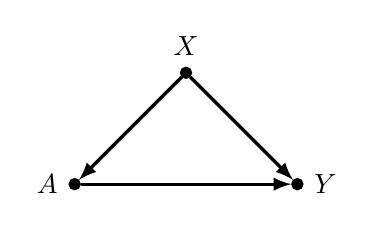
\begin{tikzpicture}[node distance = 2cm, very thick]
               \node (x)  [label = above:$X$,point];
                \node (a) [label = left:$A$ ,below left of = x , point];
                \node (y) [label = right:$Y$ ,below right of = x, point];
                % \node (u) [label = below:$(U)$ ,below right of = x, point, color = red];
                %\path[latex-latex, dashed] (z) edge[bend right = 50]  (x);
                \path (x) edge  (a);
               \path (x) edge  (y);
                \path (a) edge  (y);
                % \path (u) edge[color = red] node[below, el, color = black] {$\lambda_{ux}$} (x);
            %    \path (u) edge[color = red] node[below, el, color = black] {$\lambda_{uy}$} (y);
            % \caption{Graph $G(M)$}
        \end{tikzpicture}
 \end{center}
        \footnotesize
        \begin{itemize}
        \item<3->  Arrows go into a node only if the corresponding argument enters the corresponding function in the SCM.
        \item<4-> You could show $U_j$ pointing to each $j$, but usually omit these. 
        \end{itemize}
\end{frame}


\begin{frame}{Missing edges, bidirected arcs}
\small        
        \onslide<1-> A missing edge means the value of $A$ is not an argument into $Y$. \textit{Its the missing edges that matter for the arguments we will need to make.}\\
        \bigskip
        \begin{center}
  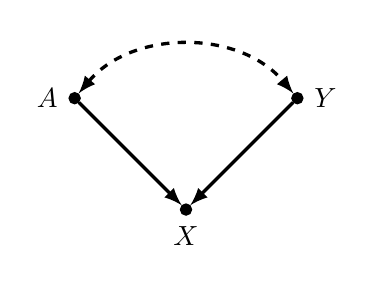
\begin{tikzpicture}[node distance = 2cm, very thick]
               \node (x)  [label = below:$X$,point];
                \node (a) [label = left:$A$, above left of = x , point];
                \node (y) [label = right:$Y$ ,above right of = x, point];
                % \node (u) [label = below:$(U)$ ,below right of = x, point, color = red];
                \path[latex-latex, dashed] (a) edge[bend left = 50]  (y);
                \path (a) edge  (x);
               \path (y) edge  (x);
        \end{tikzpicture}
\end{center}
        \onslide<2-> Some authors show unobserved common causes as a bidirected arc. \\
\end{frame}

\begin{frame}{Terminology}
\begin{enumerate}
\item<1-> nodes, vertices: the variables that are written
\item<2-> edges, arrows: the lines,  may be ``directed'' or ``bidirected'' (arcs)
\item<3-> parents: for a given node, the causes feeding into it
\item<4-> root nodes: a node with no (endogenous) parents on the graph
\item<5-> descendants, children: effects of a given cause
\item<6-> paths: any series of connected nodes, regardless of direction
\item<6-> \textbf{d}irected \textbf{a}cyclic \textbf{g}raph: a graph where all edges are directed and you can never follow directed paths from a node back to itself.
\end{enumerate}
\end{frame}

%\begin{frame}{Factorization}
%\small
%\textcolor{blue}{Markov condition}: each node listens only to its parents:
%$$p(x_j|pa_j, q_j) = p(x_j|pa_j)$$\\
%where $q_j$ are non-parents that are also non-descendants.\\ \medskip
%\onslide<2-> We'll often use this to find conditional independence or ``blocking''
%\[ X_j \indep Q_j \mid PA_j  \]\\
%
%\onslide<3-> Slang: PA ``blocks'' the relationship between $X_j$ and $Q_j$ \\
%
%\onslide<4-> Further, this allows ``Markov factorization'' of the joint distribution:
%\begin{arule}
%\footnotesize
%Product Decomposition (Pearl \& Verma 1991):  for any model $M$ whose graph $G$ is acyclic and without dependent unobserved causes (i.e. no bidirected arcs; Markovian), the joint distribution of variables in the model is given by
%\[ P(x_1, x_2, ... , x_n) =  \prod_i P(x_i | pa_i)  \]
%where $pa_i$ is the value of the parents of $X_i$
%\end{arule}
%\end{frame}
%
%\begin{frame}{Example of Product Decomposition}
%\begin{center}
%\begin{tikzpicture}
%\node[text centered] (A) {$A$};
%\node[right = 1 of A, text centered] (B) {$B$};
%\node[right=1 of B, text centered] (C) {$C$};
%% edges %
%\draw[->, line width= 1] (A) --  (B);
%\draw [->, line width= 1] (B) -- (C);
%\end{tikzpicture}
%\end{center}
%
%\small
%What is $P(A,B,C)$?  \\
%\medskip
%\onslide<2-> Without the graph, you could always write
%\[ P(A, B, C) = P(A) P(B|A) \textcolor{blue}{P(C|B, A)}  \] 
%\medskip 
%\onslide<3-> With the graph we can write:\\
%\[ P(A, B, C) = P(A) P(B|A) \textcolor{blue}{P(C|B)}  \] 
%\end{frame}

% Problem set:  study question 1.4.1 from  ``Primer''
%
%\begin{frame}{SCM--Graph}
%\small
%\begin{itemize}
%\item Every SCM ($M$) is associated with a graphical causal model  ($G$), with nodes $U$ and $V$ representing unobserved/exogeneous and observed/endogeneous causes.
%\medskip
%\item If in $M$ the function $f_X$ contains $Y$ as an argument, there will be a direct edge from $Y$ to $X$. 
%\medskip
%\item This relationship allows us to define causality graphically: in graph $G$,
%\begin{itemize}
%\item if $X$ is a child of $Y$, then $Y$ is a direct cause of $X$. 
%\item if $X$ is a descendant of $Y$, then $Y$ is a potential cause of $X$ (there are exceptions known as intransitive cases)
%\end{itemize}
%\end{itemize}
%\end{frame}

% problemt set:  study questions 1.5.1 in Primer.



\begin{frame}{Paths, dependencies, and information}  
\onslide<1-> The first use of graphs is to get a handle on what observables will be conditionally or marginally associated with what others. \\

\medskip

\onslide<2-> Three key structures: forks, chains, colliders \\

\medskip

\onslide<2-> \textcolor{Blue}{Chain}:
\begin{center}
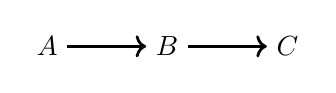
\begin{tikzpicture}
\node[text centered] (A) {$A$};
\node[right = 1 of A, text centered] (B) {$B$};
\node[right=1 of B, text centered] (C) {$C$};
% edges %
\draw[->, line width= 1] (A) --  (B);
\draw [->, line width= 1] (B) -- (C);

\end{tikzpicture}
\end{center}

\onslide<3-> Implications:\\
\medskip
 \onslide<4-> $A \indep C$ ? \\
 \medskip
\onslide<5-> $A \indep C | B$? \\
\medskip
\onslide<6-> $ B \indep C | A $? 
\end{frame}

\begin{frame}{Paths, dependencies, and information}  

\onslide<1-> \textcolor{Blue}{Fork} (aka common cause): 
\begin{center}
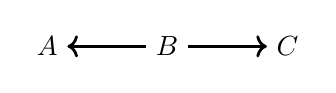
\begin{tikzpicture}
\node[text centered] (A) {$A$};
\node[right = 1 of A, text centered] (B) {$B$};
\node[right=1 of B, text centered] (C) {$C$};
% edges %
\draw[->, line width= 1] (B) --  (A);
\draw [->, line width= 1] (B) -- (C);
\end{tikzpicture}
\end{center}

\onslide<2-> Implications:\\
\medskip
 \onslide<3-> $A \indep C$ ? \\
 \medskip
\onslide<4-> $A \indep C | B$? \\
\medskip
\onslide<5-> $ B \indep C | A $? 
\end{frame}

\begin{frame}{Paths, dependencies, and information}  

\onslide<1-> \textcolor{Blue}{Collider}: 
\begin{center}
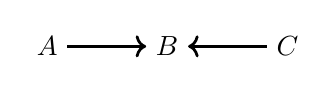
\begin{tikzpicture}
\node[text centered] (A) {$A$};
\node[right = 1 of A, text centered] (B) {$B$};
\node[right=1 of B, text centered] (C) {$C$};
% edges %
\draw[->, line width= 1] (A) --  (B);
\draw [->, line width= 1] (C) -- (B);
\end{tikzpicture}
\end{center}

\medskip
 \onslide<2-> $A \indep C$ ? \\
 \medskip
\onslide<3-> $A \indep C | B$? \\
\medskip
\onslide<4-> $ B \indep C | A $? 
\begin{center}
\textcolor{Red}{Beware colliders!}
\textcolor{Red}{Beware descendants of colliders!}
\end{center}
\end{frame}

\begin{frame}{Colliding is real}
 \footnotesize
\onslide<1-> Pearl's favorite: \\
\begin{itemize}
\item[] A: It rains
\item[] B: Sprinkler recently on
\item[] C: The lawn is wet 
\end{itemize}
\bigskip
\onslide<2-> Hollywood success:\\
\begin{itemize}
\item[] A. Good looks
\item[] B. Acting skills
\item[] C. Fame
\end{itemize}
\bigskip
\onslide<3-> Academic tenure:\\
\begin{itemize}
\item[] A: Productivity
\item[] B: Originality 
\item[] C: Tenure\footnote{Thanks to Jason Roy for these examples}
\end{itemize}
\end{frame}

\begin{frame}
\begin{figure}[h!]
\begin{center}

\includegraphics[scale=0.45]{Free Throw Percentage vs Height.png}
\end{center}
\end{figure}

%\onslide<2-> Why do you think that is? Answer with a DAG. \\
\medskip
\footnotesize
*Source: Adam Rohde, via \url{https://www.basketball-reference.com/} and \url{https://www.kaggle.com/datasets/drgilermo/nba-players-stats}.
\end{frame}


\begin{frame}{$d$-Separation}
\small 
You now understand  $d$ (directional)-Separation, which just follows from these to formalize when we can claim conditional independence

\onslide<2->
\begin{arule}
\textbf{d-separation}. \\ $A$ and $C$ are $d$-separated by a set of nodes $Z$ if  and only if:\\
\begin{itemize}
\item $A$ and $C$ are connected by a chain ($A \rightarrow B \rightarrow C$) or fork ($A \leftarrow B \rightarrow C$) s.t. $B \in Z$, or
\item $A$ and $C$ are connected by a collider ($A \rightarrow B \leftarrow C$) s.t.  the collision node is not in $Z$, and no descendant of it is in $Z$. 
\end{itemize}
\end{arule}

\onslide<3->  If nodes $A$ and $C$ are $d$-separated by $Z$, we expect $A \indep B \mid Z$ in any dataset generated by that graph. The opposite is usually, but not always, true. \\
\end{frame}

\begin{frame}{Warning: words that sound alike}
Just in case you did not notice, conditional \textcolor{Blue}{independence} is not to be confused with conditional \textcolor{Green}{ignorability}
\medskip
\begin{itemize}
\item<2-> Conditional independence is about observables, e.g. $D \indep Y | X$
\smallskip
\item<3-> Conditional ignorability is about potential outcomes, e.g. $D \indep Y_d | X$. 
\end{itemize}
\medskip
\onslide<4->  We will soon use conditional \textcolor{Blue}{independence} on DAGs to support claims of conditional \textcolor{Green}{ignorability}, but not yet. %the ``backdoor criterion'', which asks ``would $D$ and $Y$ be conditional \textbf{independent} (d-separated)''  after removing any effect of $D$ on $Y$, which will be a way to ask about $D \indep Y_d |X$...but we aren't there yet.

\end{frame}

\begin{frame}{Practice}
\begin{center}
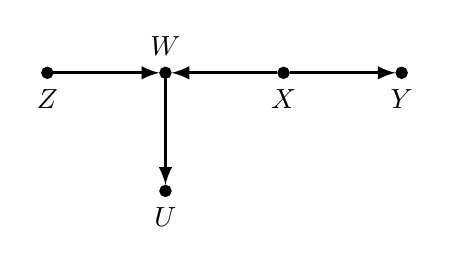
\begin{tikzpicture}[very thick]
	\node (z)  [label = below:$Z$, point];
	\node (w) [label = above:$W$ ,right of = z , point];
    \node (x) [label = below:$X$ , right of = w, point];
    \node (y) [label = below:$Y$ ,right of = x , point];
   \node (u) [label = below:$U$ ,below of = w, point];
             \path (z) edge  (w);
               \path (x) edge  (w);
                \path (w) edge  (u);               
               \path (x) edge  (y); 
\end{tikzpicture}
\end{center}

\onslide<2->  Looking at $Z$ and $Y$:
\begin{itemize}
\item Are they $d$-separated conditional on $\{\}$?
\item Are they $d$-separated conditional on $W$?
\item Are they $d$-separated conditional on $\{W,X\}$?
\item Are they $d$-separated conditional on $U$?
\end{itemize}
\end{frame}

\begin{frame}{More practice}
\begin{center}
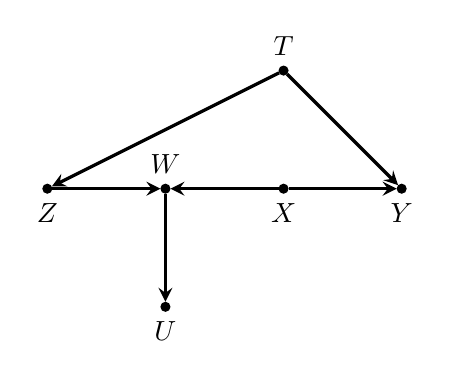
\begin{tikzpicture}
	\node (z)  [label = below:$Z$, point];
	\node (w) [label = above:$W$ ,right of = z, point];
    \node (x) [label = below:$X$, right of = w, point];
    \node (y) [label = below:$Y$ , right of = x , point];
   \node (u) [label = below:$U$ , below of = w , point];
   \node (t) [label= above:$T$, above of = x, point];
   \draw[->, >=stealth, very thick] (z) --  (w);
   \draw[->, >=stealth, very thick] (x) -- (w);
      \draw[->, >=stealth, very thick] (w) -- (u);
   \draw[->, >=stealth, very thick] (x) -- (y);
   \draw[->, >=stealth, very thick] (t) -- ( z);
   \draw[->, >=stealth, very thick] (t) -- (y);
\end{tikzpicture}
\end{center}

\onslide<2-> What sets $d$-separate $Z$ from $Y$?
\end{frame}

\begin{frame}{Review so far: }

\begin{itemize}
\small
\item<2-> Two variables come to be associated due to
\begin{itemize}
\item one causing another (directly or through a chain)
\item a common cause
\item conditioning on a common consequence (collider) 
\end{itemize}
\smallskip
\item<3-> You can render them independent ($d$-separated) if,
\begin{itemize}
\item they are independent already
\item you condition on common cause or intermediate variable
\item you don't condition on collider (or descendant thereof)
\end{itemize}
%\bigskip
%\onslide<4-> All of this is really a tool for enumerating the ways two variables can become associated, which we will later use to distinguish ``causal'' associations of interest from ``spurious'' ones. \\
%\item<4-> $d$-separation guarantees conditional independence; non-d-separation risks lack of independence.
\end{itemize}
\end{frame}

%
%\section{Interventions}
%
%\begin{frame}{Doing vs. Seeing}
%\onslide<1-> To rigorously handle causal questions we need a notation and method for imagining what interventions to a system will do to the distribution of variables. \\
%\bigskip
%\onslide<2-> \textcolor{Blue}{The cardinal sin of causal inference}: assuming that ``how the whole distribution would look if we \textit{made} $D=d$'' is the same as ``the distribution we see in the part of the data where $D=d$ already.''\\
%\bigskip
%\onslide<3-> \begin{quote}
%When we intervene on a variable in a model, we fix its value. We \textit{change} the system, and the values of other variables often change as a result. When we condition on a variable, we change nothing; we merely narrow our focus to the subset of cases in which the variable takes the value we are interested in. What changes, then, is our perception about the world, not the world itself. (\textit{Primer})
%\end{quote}
%\end{frame}
%
%\begin{frame}{More takes on seeing vs. doing}
%\onslide<1-> When you intervene, you break the very system that generated the observed data, so don't expect the observed data to tell you what would happen (without further assumptions). \\
%\bigskip
%\onslide<2-> Often easier to think in terms of comparisons (e.g. $X=x$ vs. $X=x'$):\\
%\small
%\begin{itemize} 
%\item when you compare $p(Y|X=x)$ to $p(Y|X=x')$, these groups differ on things besides $X$ (e.g. those things that influenced $X$ and descendants thereof)
%\item but when you \textbf{do} $X=x$ and $X=x'$, you leave everything else up-stream of $X$ untouched and look at how $p(Y)$ differs under intervention on $X$.
%\end{itemize}
%\end{frame}
%
%
%\begin{frame}{Doing vs. Seeing}
%\onslide<1-> Enter the $do$-operator:
%\small
%\begin{itemize}
%\item<2-> $P(Y|X=x)$: the distribution of $Y$ when we saw $X=x$. 
%\item<3-> $P(Y|do(D=d))$: the distribution of $Y$ if everybody in the population had $D$ set to $d$.
%\item<4-> Might be clearer to say $P_{do(D=d)}(Y)$, since you are \textit{not} conditioning
%\end{itemize}
%
%\normalsize
%\onslide<5-> For example,\\
%\small
%\begin{itemize}
%\item<5-> For $Y$, distributional result under intervention: $P(Y=y|do(X=x))$, \textcolor{Red}{not} $P(Y|X=x)$.
%\smallskip
%\item<6-> For all observables ($V$), distribution had you intervened to make $X=x$: $P(V|do(X=x))$, not $P(V|X=x)$.
%\smallskip
%\item<7-> A single individual's value of $Y$ under intervention: $f_y(X=x, U=u_i)$...i.e. potential outcome, $Y_i(x)$
%\end{itemize}
%\end{frame}
%
%\begin{frame}{No side-effects:}
%\onslide<1-> Intervening in this way is assumed to be free of ``side-effects'' -- 
%
%\small
%\begin{itemize}
%\item the act of assigning $X=x$ does not alter the outcome except through the assigned value of $X$ and the consequences of this governed by the SCM.
%\smallskip
%\item e.g. if being forced to take a vaccine as opposed to taking it by choice makes somebody angry at the government and they then stop wearing a mask...you can do this but you'd have to have all that on the graph.
%\smallskip
%\item here this is down to ``modularity''/``invariance''; similar notion with POs was managed through consistency and ``no multiple versions of treatment'' assumption (forced treatment is different from volitional treatment).
%\smallskip
%\item In other words, we are trusting that intervention doesn't change the SCM/DAG except by ``resetting'' the treatment as we demand. 
%\end{itemize}
%\end{frame}
%
%\begin{frame}{Modified graphs}
%\onslide<1-> To reflect this resetting, when we $do(A=a)$ and assume no side-effects, we change the SCM (or ask about a sub-model) where:\\
%\small
%\begin{itemize}
%\item the original links from $A$'s parents into $a$ have been removed
%\smallskip
%\item $A$ is now set equal to $a$
%\smallskip
%\item typically (especially in Hernan \& Robins) we imagine setting $A$ to the same $a$ for \textit{everybody}, but you can also do different values for different units, or inspect what happens to individual units. 
%\end{itemize}
%\normalsize
%\onslide<3-> The resulting distribution is the ``interventional distribution'', consistent with the interventional graph.\\
%\begin{itemize}
%\item the identification question: can you somehow mimic this distribution using only data  generated from the observational graph?
%\end{itemize}
%\end{frame}
%
%\begin{frame}{Example of graph modification}
%Suppose you have ice cream sales ($A$), crime rates ($Y$), and temperature ($X$).   \\
%\medskip
%
%\onslide<2-> What happens when you fix $A=a$?
%
%\begin{columns}[T] % align columns
%\begin{column}{.48\textwidth}
%
%\begin{figure}
%  \begin{tikzpicture}[node distance = 2cm]
%             \node (x)  [label = right:$X$, point];
%             \node (a) [label = left:$A$ ,below left of = x , point];
%             \node (y) [label = right:$Y$ ,below right of = x, point];
%            \node (ux) [label = left:$U_x$ ,above of = x , point];
%            \node (ua) [label = left:$U_a$ ,above of = a , point];
%            \node (uy) [label = left:$U_y$ ,above of = y , point];
%                % \node (u) [label = below:$(U)$ ,below right of = x, point, color = red];
%                %\path[latex-latex, dashed] (z) edge[bend right = 50]  (x);
%                \path (x) edge  (a);
%               \path (x) edge  (y);
%                \path (ux) edge  (x);               
%               \path (ua) edge  (a);                
%                \path (uy) edge  (y);
%                % \path (u) edge[color = red] node[below, el, color = black] {$\lambda_{ux}$} (x);
%            %    \path (u) edge[color = red] node[below, el, color = black] {$\lambda_{uy}$} (y);
%            % \caption{Graph $G(M)$}
%        \end{tikzpicture}
%       \caption*{Graph $G$ of Model $M$}
%        \end{figure}
%        
%        
%\end{column}%
%\hfill%
%\begin{column}{.48\textwidth}
%\begin{figure}
%  \begin{tikzpicture}[node distance = 2cm]
%             \node (x)  [label = right:$X$, point];
%             \node (a) [label = below:$\ensuremath{A=a}$ ,below left of = x , point];
%             \node (y) [label = right:$Y$ ,below right of = x, point];
%            \node (ux) [label = left:$U_x$ ,above of = x , point];
%            \node (ua) [label = left:$U_a$ ,above of = a , point];
%            \node (uy) [label = left:$U_y$ ,above of = y , point];
%                % \node (u) [label = below:$(U)$ ,below right of = x, point, color = red];
%                %\path[latex-latex, dashed] (z) edge[bend right = 50]  (x);
%               % \path (x) edge  (a);
%               \path (x) edge  (y);
%                \path (ux) edge  (x);               
%               %\path (ua) edge  (a);                
%                \path (uy) edge  (y);
%                % \path (u) edge[color = red] node[below, el, color = black] {$\lambda_{ux}$} (x);
%            %    \path (u) edge[color = red] node[below, el, color = black] {$\lambda_{uy}$} (y);
%            % \caption{Graph $G(M)$}
%        \end{tikzpicture}
%        \caption*{Graph $G_m$ of Model $M_m$}
%        \end{figure}
%        
%\end{column}%
%\end{columns}
%\end{frame}
%
%
%
%\begin{frame}{The easy case}
%
%
%For the next while we will focus on ``complete'' or Markovian graphs -- those with no bidirected arcs/ unobserved common causes.
%
%\end{frame}
%
%\begin{frame}{Interventions}
%\onslide<1-> Let's return to our Simpson's paradox example, letting $X=gender$, $D=drug$, and $Y=recovery$:\\
%\begin{figure}
%  \begin{tikzpicture}[node distance = 2cm]
%               \node (x)  [label = above:$X$,point];
%                \node (d) [label = left:$D$ ,below left of = x , point];
%                \node (y) [label = right:$Y$ ,below right of = x, point];
%                % \node (u) [label = below:$(U)$ ,below right of = x, point, color = red];
%              %  \path[latex-latex, dashed] (Gender) edge[bend right = 50]  (Drug);
%                \path (x) edge  (d);
%               \path (x) edge  (y);
%                \path (d) edge  (y);
%                % \path (u) edge[color = red] node[below, el, color = black] {$\lambda_{ux}$} (x);
%            %    \path (u) edge[color = red] node[below, el, color = black] {$\lambda_{uy}$} (y);
%            % \caption{Graph $G(M)$}
%        \end{tikzpicture}
%        \end{figure}
%        \onslide<2-> What is the effect of the drug?
%        \small
%        \begin{itemize}
%        \item<3-> \textcolor{Blue}{Question}:  imagine hypothetical intervention in which everybody is given the drug, compare to recovery rate under  intervention where nobody is given the drug. Average. 
%        \item<4-> \textcolor{Blue}{Answer is from distribution generated by a new model}: 
%        \[ Pr(Y=1 | do(D=1)) - Pr(Y=1 | do(D=0))\]
%        \item<5-> \textcolor{Blue}{More general ``causal effect''}: $P(Y=y|do(D=d)), \; \forall d \in D $
%        \end{itemize}
%\end{frame}
%
%\begin{frame}{Intervention and distributions}
%\onslide<1-> Plan:
%\begin{itemize}
%\item<2-> Start with your observational graph ($G$) and the implied distribution ($P$).
%\smallskip
%\item<3-> Get your modified graph ($G_m$) whose distribution ($P_m$) describes the world under $do(D=d)$. 
%\smallskip
%\item<4-> See if you can replace $P_m(Y|d)$ with quantities from $P$ only (``identification'')
%\end{itemize}
%\end{frame}
%
%\begin{frame}
%\small
%\onslide<1-> Our modified graph is:
%\begin{figure}
%  \begin{tikzpicture}[node distance = 1.5cm]
%               \node (x)  [label = above:$X$,point];
%                \node (d) [label = left:$\text{D=d}$ ,below left of = x , point];
%                \node (y) [label = right:$Y$ ,below right of = x, point];
%                % \node (u) [label = below:$(U)$ ,below right of = x, point, color = red];
%              %  \path[latex-latex, dashed] (Gender) edge[bend right = 50]  (Drug);
%               % \path (x) edge  (d);
%               \path (x) edge  (y);
%                \path (d) edge  (y);
%                % \path (u) edge[color = red] node[below, el, color = black] {$\lambda_{ux}$} (x);
%            %    \path (u) edge[color = red] node[below, el, color = black] {$\lambda_{uy}$} (y);
%            % \caption{Graph $G(M)$}
%        \end{tikzpicture}
%     \end{figure}
%     \onslide<2-> The $do$-action can be written in terms of $P_m$:
%     \footnotesize
%     \begin{align*}
%		P(Y=y | do(D=d)) &= P_m(Y=y| D=d) \quad \text{by definition} \\
%		&=   \sum_x P_m(Y=y  | D=d, X=x)   P_m(X=x)
%     \end{align*}
%     \small
%     \onslide<3-> Can we replace parts of $P_m$ with equivalents from $P$?\\
%     \footnotesize
%     \begin{itemize}
%     \footnotesize
%     \item<4-> $Y=f_y(D,X, U_y)$ in both original and $M$. Thus, $P_m(Y=y | D=d, X=x) = P(Y=y|D=d, X=x)$, \\ (i.e. dependence of $Y$ on $D$ and $X$ unchanged by intervention).
%     \item<5-> In both, $X=f_x(U_x)$, so $P_m(X) = P(X)$. (i.e. $X$ remains the same in both) \end{itemize}         
%\end{frame}
%
%\begin{frame}{Intervention continued}
%\footnotesize
%   \begin{align*}
%		P(Y=y | do(D=d)) &= P_m(Y=y| D=d) \quad \text{by definition} \\
%		&=   \sum_x P_m(Y=y  | D=d, X=x)   P_m(X=x)\\
%		&= \sum_x P(Y=y | D=d, X=x) P(X=x)
%     \end{align*}
%     \small
%     \onslide<2->  \textcolor{Blue}{Identification achieved}: only observable quantities required\\
%\end{frame}
%
%
%\begin{frame}{The Adjustment Formula}
%\small
%\onslide<1-> This example is a particular case of a general rule: the adjustment set should correspond to the parents of $D$. \\
%\medskip
%\onslide<2-> 
%\begin{arule}
%\textbf{Causal effect rule}/ adjustment formula.  Given a graph $G$ in which variables $PA$ are parents of $X$, the causal effect of $X$ on $Y$ is given by:
%\[P(Y=y|do(X=x)) = \sum_z P(Y=y |  X=x, PA=z) P(PA=z)  \]
% \end{arule}
%
%%\onslide<3-> You might like to rewrite this as:\\
%%\[ P(y|do(x)) = \sum_z \frac{P(X=x, Y=y, PA=z)}{P(X=x | PA=z)} \]
%%which describes an adjustment procedure for tables, or inverse propensity score weighting. \\
%\end{frame}
%
%
%\begin{frame}{Thinking about differences}
%\footnotesize
%\onslide<1-> Defining the causal ``effect'' as $P(Y|do(D=d))$ is awkward since we usually care about particular differences. \\ 
%
%\medskip
%\onslide<2-> We can construct contrasts using the adjustment formula with $do(D=d)$ and $do(D=d')$ \\
%\onslide<3->
%\begin{align*}
%ACE &= \E(Y=1|do(D=1)) - \E(Y=1|do(D=0)) \\
%&= \sum_x Pr(Y=1 | D=1, X=x) P(X=x) - \sum_x Pr(Y=1 | D=0, X=x) P(X=x) \\
%&= \sum_x \left[ Pr(Y=1 | D=1, X=x) - P(Y=1 | D=0, X=x) \right]  P(X=x) 
%\end{align*}
%\begin{itemize}
%\item<3-> i.e. look within each stratum of $X$ at how $Y$ differs for the treated and control  
%\item<4-> holding $X$ constant within stratum ensures association of $D$ and $Y$ is due to effect of $D$
%\item<5-> this was how we adjusted under the conditional ignorability assumption with POs.
%\end{itemize}
%\end{frame}
%
%% Study questions 3.2.1
%
%\begin{frame}{Practice and the truncated product rule}
%When you intervene on a variable, its distribution becomes a constant, which truncates the factorization. \\
%\onslide<2-> 
%\begin{columns}[T] % align columns
% \begin{column}{.48\textwidth}
%\begin{figure}
%  \begin{tikzpicture}[->,>=stealth',shorten >=1pt,auto,node distance=2cm,
%  thick,main node/.style={circle,fill=blue!20,draw,font=\sffamily\Large\bfseries}]
%  %[node distance = 1.5cm]
%               \node (x)  [label = above:$X$,point];
%                \node (d) [label = left:$D$ ,below left of = x , point];
%                \node (y) [label = right:$Y$ ,below right of = x, point];
%                % \node (u) [label = below:$(U)$ ,below right of = x, point, color = red];
%              %  \path[latex-latex, dashed] (Gender) edge[bend right = 50]  (Drug);
%                \path (x) edge  (d);
%               \path (x) edge  (y);
%                \path (d) edge  (y);
%                % \path (u) edge[color = red] node[below, el, color = black] {$\lambda_{ux}$} (x);
%            %    \path (u) edge[color = red] node[below, el, color = black] {$\lambda_{uy}$} (y);
%        \end{tikzpicture}
%         \caption{Graph $G$}
%        \end{figure}
%	\end{column}
%\begin{column}{.48\textwidth}
%\begin{figure}
%  \begin{tikzpicture}[->,>=stealth',shorten >=1pt,auto,node distance=2cm,
%  thick,main node/.style={circle,fill=blue!20,draw,font=\sffamily\Large\bfseries}]
%               \node (x)  [label = above:$X$,point];
%                \node (d) [label = left:$\text{D=d}$ ,below left of = x , point];
%                \node (y) [label = right:$Y$ ,below right of = x, point];
%                % \node (u) [label = below:$(U)$ ,below right of = x, point, color = red];
%              %  \path[latex-latex, dashed] (Gender) edge[bend right = 50]  (Drug);
%               % \path (x) edge  (d);
%               \path (x) edge  (y);
%                \path (d) edge  (y);
%                % \path (u) edge[color = red] node[below, el, color = black] {$\lambda_{ux}$} (x);
%            %    \path (u) edge[color = red] node[below, el, color = black] {$\lambda_{uy}$} (y);
%        \end{tikzpicture}
%        \caption{Graph $G_m$}
%     \end{figure}
%     \end{column}
%\end{columns}
%\small
%\onslide<3-> What joint distribution does $G$ produce?  $P(d,x,y) = P(x)P(d|x)P(y|d,x)$\\
%\medskip
%\onslide<4-> How about $G_m$?\\
%\vspace{-.1in}
%\begin{align*}
%P(x,y|do(d)) &= P_m(x) \text{\sout{\ensuremath{P_m(d|x)}} }  P_m(y|d,x)  \\
%&= P(x)P(y|d,x)  
%\end{align*}
%\end{frame}
%
%
%\begin{frame}{Practice and the truncated product rule}
%\vspace{-.5in}
%\begin{columns}[T] % align columns
% \begin{column}{.48\textwidth}
%\begin{figure}
%  \begin{tikzpicture}[node distance = 1.5cm]
%               \node (x)  [label = above:$X$,point];
%                \node (d) [label = left:$D$ ,below left of = x , point];
%                \node (y) [label = right:$Y$ ,below right of = x, point];
%                % \node (u) [label = below:$(U)$ ,below right of = x, point, color = red];
%              %  \path[latex-latex, dashed] (Gender) edge[bend right = 50]  (Drug);
%                \path (x) edge  (d);
%               \path (x) edge  (y);
%                \path (d) edge  (y);
%                % \path (u) edge[color = red] node[below, el, color = black] {$\lambda_{ux}$} (x);
%            %    \path (u) edge[color = red] node[below, el, color = black] {$\lambda_{uy}$} (y);
%        \end{tikzpicture}
%         \caption{Graph $G$}
%        \end{figure}
%	\end{column}
%\begin{column}{.48\textwidth}
%\begin{figure}
%  \begin{tikzpicture}[node distance = 1.5cm]
%               \node (x)  [label = above:$X$,point];
%                \node (d) [label = left:$\text{D=d}$ ,below left of = x , point];
%                \node (y) [label = right:$Y$ ,below right of = x, point];
%                % \node (u) [label = below:$(U)$ ,below right of = x, point, color = red];
%              %  \path[latex-latex, dashed] (Gender) edge[bend right = 50]  (Drug);
%               % \path (x) edge  (d);
%               \path (x) edge  (y);
%                \path (d) edge  (y);
%                % \path (u) edge[color = red] node[below, el, color = black] {$\lambda_{ux}$} (x);
%            %    \path (u) edge[color = red] node[below, el, color = black] {$\lambda_{uy}$} (y);
%        \end{tikzpicture}
%        \caption{Graph $G_m$}
%     \end{figure}
%     \end{column}
%\end{columns}
%\footnotesize
%\onslide<2-> This recovers the adjustment formula: 
%\[ P(y|do(d)) = \sum_x P(x)P(y|d,x) \]
%\onslide<3-> You might rewrite this wrt to strata:
%\[ P(x,y,do(d)) = \frac{P(d,y,x)}{P(d|x)} \]
%I.e. to adjust a frequency table for $P(d,y,x)$ based on $do(D=d)$, just divide each cell by $P(d|x)$ (the propensity score).  \\
%\smallskip
%
%\onslide<3-> After that, you can marginalize and do contrasts as you'd like. 
%\end{frame}
%
%
%\begin{frame}{Multiple interventions and truncated product rule}
%\small
%\onslide<1-> Let's codify this, and consider multiple treatments \\
%\smallskip
%\begin{theorem}
%\textbf{Truncated product rule or g-formula} Under interventions that fix a set of variables $X$ to constants:\\
%\[P(x_1, x_2, ..., x_n | do(x)) = \prod_i P(x_i | pa_i),  \quad \forall \; i \; \text{with}\; X_i \; \text{not in}\; X \] 
%\end{theorem}
%
%\onslide<2-> Just delete from the expansion any thing that is parentless (intervened on) in the modified graph. \\
%\end{frame}
%
%\begin{frame}{Example of multiple interventions}
%\begin{figure}[h]
%\begin{center}
%\epsfig{figure=r391-fig2a-edit.eps,width=1.75in} 
%\end{center}
%\end{figure}
%\onslide<1-> Set $X$ to $x$ and $Z_3$ to $z_3$. What is the post-intervention distribution over the remaining variables?\\
%\smallskip
%\onslide<2->
%\[P(z_1, z_2, w, y | do(X=x, Z_3=z_3)) =  P(z_1)P(z_2)P(w|x)P(y|w,z_3,z_2) \]
%%\onslide<3-> Again, factoring as per the modified graph, which deletes $P_m(x|z_1,z_3)$ and $P_m(z_3|z_1, z_2)$ from the product. \\ 
%\end{frame}
%
%\section{Identification with partial graphs}
%\begin{frame}{Mission accomplished?}
%\small
%\onslide<1-> We have solved all of causal inference, right?! \\
%\footnotesize
%\begin{itemize}
%\item<2-> Use a graph (but really only) to find the parents of the treatment, then use adjustment formula
%\end{itemize}
%
%\medskip
%\small
%\onslide<3->  Not so fast! \\
%\footnotesize
%\begin{itemize}
%\item Often, some parents of treatment will be unobserved so you can't just use these rules, yet there are ID options.
%\end{itemize}
%\small
%\onslide<4->\textcolor{Blue}{Question}: given a (possibly partial) graph, can we estimate a causal effect of one variable on another, and what variables should we adjust for to do so? \footnotesize
%\begin{itemize}
%\item<5-> The ``$do$-calculus'' gives rules for converting $do$ statements into $do$-free statements, adding some tricks to what we've seen above.
%\item<6-> However many cases can be covered by a simple graphical criterion: the backdoor criterion while another set is covered by front-door criterion.
%\end{itemize}
%\end{frame}

\subsection{Backdoor Criterion}

\begin{frame}{Frontdoor paths and backdoor paths}
\small
\begin{itemize}
\item<2-> A \textcolor{Blue}{frontdoor path} from $D$ to $Y$ begins with an arrow emanating out of $D$. 
\begin{itemize}
\footnotesize
\item These carry effects of treatment, so usually we do not want to block these.
\end{itemize}
\small
\item<3-> \textcolor{Blue}{Backdoor paths} between $D$ and $Y$ point into $D$. 
\begin{itemize}
\footnotesize
\item These are typically unwanted sources of association we will want to remove from what we measure.
\end{itemize}
\end{itemize}
\end{frame}


\begin{frame}{Frontdoor paths and backdoor paths}
\small
\onslide<1-> The  \textbf{backdoor criterion}:\\
\begin{itemize} \setlength\itemsep{1em}
\item<2-> choose variables $\{Z\}$ that can block all backdoor paths from treatment to outcome, without including any descendants of treatment.
\item<3-> (equivalent ``trick'':  remove arrows out of $D$ on your graph, and find $\{Z\}$ that can d-separate $D$ and $Y$.)
\item<4-> if you can do this, you can \textcolor{Blue}{identify the effect} of $D$ on $Y$ by conditioning on those $\{Z\}$.
\item<5-> it also means you obtained $Y_d \indep D | \{Z\}$, i.e. conditional ignorability, SOO. (more in a moment)
\item<6-> in more natural terms: if you rule out ``spurious'' reasons for such an association, then you have only the causal reason left. 
\end{itemize}
\onslide<7-> This is 93+\% of what people use DAGs for.\\
\end{frame}


%\begin{frame}{Backdoor criterion}
%\small
%\onslide<2-> \begin{definition}
%\textbf{Backdoor criterion}: Given an ordered pair of variables ($X$,$Y$) in a directed acyclic graph $G$, a set of variables $Z$ satisfies the \textit{backdoor criterion} relative to ($X$,$Y$) if no node in $Z$ is a descendant of $X$, and $Z$ blocks every path between $X$ and $Y$ that contains an arrow into $X$.
%\end{definition}
%\onslide<3-> For humans: condition on a set of nodes $Z$ s.t.:
%\begin{enumerate}
%\item you block all spurious (backdoor) paths between $X$ and $Y$
%\item you leave all directed (frontdoor) paths from $X$ to $Y$ unchanged
%\item don't open new spurious paths (i.e. through conditioning on collider or its descendants)
%\end{enumerate}
%
%\onslide<4-> \textcolor{Blue}{Preview}: backdoor criterion given $\{Z\} \implies Y_d \indep D | Z$...but that's for later. 
%\end{frame}

\begin{frame}{What next?}
\onslide<1-> Once you find a conditioning set $Z$ that satisfies the backdoor criterion relative to $D$ on $Y$, you can\\
\small
\begin{itemize}
\item<2-> In DAG land:  compute $p(Y|do(d))$ using the adjustment formula, $$p(Y|do(d))=\sum_z p(Y|d,z)p(z)$$
\begin{itemize}
\item<3-> This is very general; you are more used to asking for the ATE, which you can get from this:
\begin{align*}
\scriptsize
\E[Y_1-Y_0] &= \sum_z y*p(Y=y|d=1,z)p(z)-\sum_z y*p(Y=y|d=0,z)p(z)  \\
&= \sum_z (\E[Y|d=1,z]-\E[Y|d=0,z])p(z) \\
&= \text{our usual approach under SOO}
\end{align*}

\end{itemize} 
\item<4-> In PO land: ``you have shown SOO/CI, so condition on $Z$'', i.e. estimate treatment effect within strata of $Z$, average over strata.
\item<5-> In practice: use your favorite technology to ``adjust for'' $Z$.
\end{itemize}
\end{frame}

\begin{frame}{Example 1}
\onslide<1-> 
\begin{center}
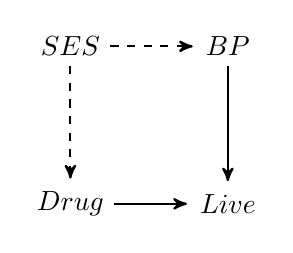
\begin{tikzpicture}[-,>=stealth',shorten >=1pt,auto,node distance=2cm,
  thick,main node/.style={circle,fill=blue!20,draw,font=\sffamily\Large\bfseries}]
  \node (x) {$Drug$};
  \node (z) [above of=x] {$SES$};
  \node (w) [right of=z] {$BP$};
  \node (y) [right of=x] {$Live$};
  \draw[->] (x) -- (y);
  \draw[->] (w) -- (y);
  \draw[dashed, ->] (z) -- (x);
  \draw[dashed, ->] (z) -- (w);
\end{tikzpicture}
\end{center}
where $SES$ is socioeconomic status (unobserved), $BP$ is blood pressure, $Drug$ is a treatment, and $Live$ is the outcome. 
\footnotesize
\begin{itemize}
\item<2-> Go for backdoor criterion: what do you choose?
\item<3-> Condition on it. 
\end{itemize}
\end{frame}
%
%\begin{frame}{Try it by factoring to verify:}
%\footnotesize
%\begin{align*}
%P(Live|do(Drug=d)) &= P_m(Live|Drug=d) \\
%&=  \sum_{BP, SES}  P_m(Live| BP, Drug=d, SES) P_m(BP|SES)P_m(SES) \\
%&=  \sum_{BP, SES}  P_m(Live| BP, Drug=d) P_m(BP|SES)P_m(SES) \\
%&= \sum_{BP} P_m(Live | BP, Drug=d) P_m(BP) \\
%&= \sum_{BP} P(Live|BP, Drug=d)P(BP)
%\end{align*}
%\onslide<3-> This is the long way around to what backdoor told you to do. \\
%\medskip
%\onslide<4-> Not always this easy though, which is why the do-calculus exists.
%\end{frame}

%\begin{frame}{Invariance of nature to estimation}
%\small
%\onslide<1-> Remember the $P(Y|do(Drug))$ we are trying to recovery has to be estimated but is itself a fact of nature. \\
%\bigskip
%\begin{itemize}
%\item Suppose you have more than one way to estimate a causal effect (e.g. if $SES$ had been observed)
%\item  You should get the same result regardless of which you choose (up to finite sample problems) 
%\item  If you don't, then your model is wrong. 
%\item I.e. a multiplicity of valid conditioning sets gives testable implications of model.
%\end{itemize}
%\end{frame}

%\begin{frame}{A tricky example}
%p62/63 has example where you shouldn't condition but then if you want conditional effect, %conditioning will bias, so you have to condition on other things. 
%\end{frame}


\begin{frame}{Example 2}
\small
\begin{figure}
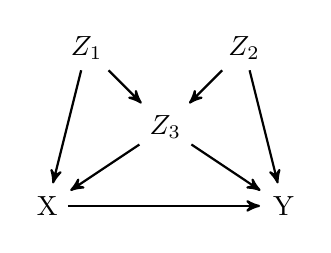
\begin{tikzpicture}[->,>=stealth',shorten >=1pt,auto,node distance=2cm,
  thick,main node/.style={circle,fill=blue!20,draw,font=\sffamily\Large\bfseries}]
\node at (0,0) (X) {X};
\node at (3,0) (Y) {Y};
\node at (.5,2) (Zone) {$Z_1$};
\node at (2.5,2) (Ztwo) {$Z_2$};
\node at (1.5,1) (Zthree) {$Z_3$};
\draw[->, line width=.8] (X) -- (Y);
\draw[->, line width=.8] (Zone) -- (X);
\draw[->, line width=.8] (Ztwo) -- (Y);
\draw[->, line width=.8] (Zone) -- (Zthree);
\draw[->, line width=.8] (Ztwo) -- (Zthree);
\draw[->, line width=.8](Zthree) -- (X);
\draw[->, line width=.8](Zthree) -- (Y);
\end{tikzpicture}
\end{figure}
\begin{itemize}
\item<2-> What are the backdoor paths from $X$ to $Y$?
\item<3-> What sets block them?
\end{itemize}
\end{frame}

% Other good practice examples can be found on Coursera course. 
%
%\begin{frame}{Disjunctive Cause Criterion (VanderWeele 2011)}
%%\small (also  Confounder selection criterion (VanderWeele and Shpitser 2011))\\
%%\medskip
%\onslide<1-> A partial graph criterion: \\
%\begin{arule}
%\textbf{Disjunctive Cause Criterion}(VanderWeele 2011). 
%\footnotesize
%If (1) there is a set of observed variables that satisfy backdoor criterion, then (2) a subset that 
%includes all (observed) causes of the exposure, the outcome, or both will be sufficient for adjustment. 
%\end{arule}
%\bigskip
%\small
%\onslide<2-> But you need to know if a set satisfying the backdoor criterion exists, so not always helpful. 
%\end{frame}
%
%\begin{frame}{What does disjunctive cause criterion tell you here?}
%\begin{figure}
%\begin{tikzpicture}[->,>=stealth',shorten >=1pt,auto,node distance=2cm,
%  thick,main node/.style={circle,fill=blue!20,draw,font=\sffamily\Large\bfseries}]
%\node at (0,0) (X) {X};
%\node at (3,0) (Y) {Y};
%\node at (.5,2) (Zone) {$Z_1$};
%\node at (2.5,2) (Ztwo) {$Z_2$};
%\node at (1.5,1) (Zthree) {$Z_3$};
%\draw[->, line width=.8] (X) -- (Y);
%\draw[->, line width=.8]  (Zone) -- (X);
%\draw[->, line width=.8] (Ztwo) -- (Y);
%\draw[->, line width=.8] (Zone) -- (Zthree);
%\draw[->, line width=.8] (Ztwo) -- (Zthree);
%\draw[->, line width=.8](Zthree) -- (X);
%\draw[->, line width=.8](Zthree) -- (Y);
%\end{tikzpicture}
%\end{figure}
%\end{frame}


\begin{frame}{How about here?}
\begin{figure}
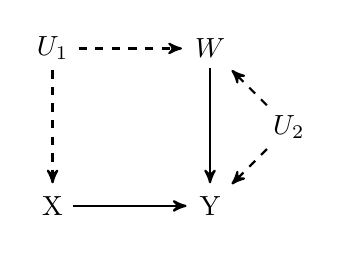
\begin{tikzpicture}[->,>=stealth',shorten >=1pt,auto,node distance=2cm,
  thick,main node/.style={circle,fill=blue!20,draw,font=\sffamily\Large\bfseries}]
\node at (0,0) (X) {X};
\node at (2,0) (Y) {Y};
\node at (0,2) (Uone) {$U_1$};
\node at (2,2) (W) {$W$};
\node at (3,1) (Utwo) {$U_2$};
\draw[->, line width=.8] (X) -- (Y);
\draw[->, line width=.8] (W) -- (Y);
\draw[dashed, ->] (Uone) -- (X);
\draw[dashed, ->] (Uone) -- (W);
\draw[dashed, ->] (Utwo) -- (W);
\draw[dashed, ->] (Utwo) -- (Y);
\end{tikzpicture}
\end{figure}
\end{frame}

% Problem set -- study question 3.3.1

\subsection{Adjustment Criterion}
\begin{frame}{Adjustment Criterion}
\onslide<1-> Shpitser, VanderWeele,  Robins (2012) \\
\bigskip
\onslide<2-> Noting that  $G_{\overline{x}}$ is the graph representing $do(X=x)$\footnote{Also relevant: this paper defines descendants of $X$ to include $X$ itself.} 
\begin{arule}
\textbf{Adjustment criterion.} $Z$ satisfies the adjustment criterion relative to $(X,Y)$ in  $G$ if
(i) No element in $Z$ is a descendant in $G_{\overline{x}}$ of any $W \notin X$ which lies on a proper causal path from $X$ to $Y$; (ii) All non-causal paths in $G$ from $X$ to $Y$ are blocked by $Z$.
\end{arule}

\onslide<3-> Basically backdoor criterion, but allows conditioning on descendants of $X$ when it is not on path to $Y$.
\end{frame}

\begin{frame}{Adjustment criterion vs. Backdoor}
\small
\onslide<1-> Example:
\begin{center}
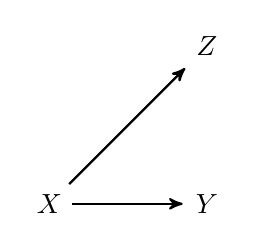
\begin{tikzpicture}[-,>=stealth',shorten >=1pt,auto,node distance=2cm,
  thick,main node/.style={circle,fill=blue!20,draw,font=\sffamily\Large\bfseries}]
  \node (x) {$X$};
  \node (y) [right of=x] {$Y$};
  \node (z) [above of=y] {$Z$};
  \draw[->] (x) -- (y);
  \draw[->] (x) -- (z);
\end{tikzpicture}
\end{center}

\onslide<2-> Conditioning on $Z$  fails backdoor for effect of $X$ on $Y$, but not adjustment criterion. \\
\medskip
\footnotesize
\begin{itemize}
\item<3-> If it satisfies the backdoor criterion, it satisfies the adjustment criterion. 
\item<4-> Further, this is complete in that if $Z$ fails to satisfy the adjustment criterion, then adjusting for $Z$ will fail to produce a valid effect estimate.
\item<5-> I don't know when this is useful in practice, but it is complete.
\item<6-> Conditioning on such a $Z$ could also weaken estimation, since conditionally on $Z$, variation in $X$ would be lessened.
\end{itemize}
\end{frame}


\begin{frame}{DAGs, POs, and conditional ignorability}
Again, \\
\onslide<1-> \begin{center}
\textcolor{Red}{If some $\{Z\}$ satisfies backdoor/adjustment criterion for Y-D, then $Y_d \indep D \mid  \{Z\}$ (conditional ignorability)} \end{center}
\small
\onslide<2-> We won't show this rigorously, but try this on:
\begin{itemize}
\item<3-> ``Satisfying backdoor means that, conditional on $\{Z\}$, there is no reason $Y$ and $D$ are related but for the effect of $D$ on $Y$.''
\item<4->  ``If, within strata of $\{Z\}$, you thought the only way $D$ and $Y$ were related was through the effect of treatment (i.e. backdoor holds), then within strata of $\{Z\}$, you'd have $Y_0$ independent of $D$. To help, you can imagine that looking at $Y_0$ ``removes from $Y$ the effect of $D$''.
\end{itemize}

\begin{itemize}\setlength\itemsep{1em}
\item<5-> Mostly people use DAGs just to check if conditioning on some $\{Z\}$ is a good idea, or to choose the $\{Z\}$ to condition on.
\item<6-> DAGs and POs are compatible; DAGs help find failures in conditional ignorability claims. They are a thinking aid.
\end{itemize}
\end{frame}

\section{DAG Revelations}

\begin{frame}{Why bother? Some errors and revelations made clear by DAGs}
\begin{itemize} \setlength\itemsep{1em}
\item  M-bias, butterfly bias, sample selection
\item Stratifying on post-treatment variables
\item Why you cannot control for Z and check D-Y for exclusion restriction.
%\item Front-door criterion
%\item maybe one time-series thing?
%\item daggity/ causal fusion. 
\end{itemize}
\end{frame}

%
\begin{frame}
\frametitle{M-bias, butterly bias, sample selection}
%\small
You already saw this but let's do another example\footnote{Example and ggdag code courtesy of Malcolm Barrett, using an example borrowed from ``Modern Epidemiology''}
\footnotesize
\begin{figure}[h!]
\begin{center}

\includegraphics[scale=.45]{mbias.pdf}
\end{center}
\end{figure}
\end{frame}


\begin{frame}
\frametitle{Stratifying on post-treatment trouble}
\begin{figure}[h!]
\begin{center}

\includegraphics[scale=.3]{newschool.pdf}
\end{center}
\end{figure}
\end{frame}

\begin{frame}
\frametitle{You can't show exclusion by checking $Y \sim Z | D$}
\begin{figure}[h!]
\begin{center}

\includegraphics[scale=.25]{iv.pdf}
\end{center}
\end{figure}
\end{frame}

%
\section{Complaints and responses}

\begin{frame}{}
1. I can't hope to know the whole causal structure, so I prefer to just focus on POs. \\

\medskip

\onslide<2-> Sorry, life really is that hard. The PO-based claims you'd like to make (e.g. CI/SOO) can be wrong due to the causal structure, so you can't wish it away. e.g.:\\
\medskip
\small
\begin{itemize} \setlength\itemsep{1em}
\item<3-> If you can think of a plausible DAG that would not satisfy backdoor, there is a problem your CI story.
\item<4-> Given colliders and such, this enables you to find challenges to CI that are not obvious
\end{itemize}
\end{frame}

\begin{frame}{}
2. Many ID strategies (IV, RDD, DID) depend on assumptions not on a DAG, and therefore cannot be ``proven'' or fully understood from DAG perspective.
\small
\begin{itemize}
\item Good reason to be bilingual and not \textit{just} rely on DAGs. 
\item But these approaches still require assumptions that can be shown on DAG \textit{plus} some others, so you can still surface problems from the DAG side
\item In fact DAGs are great for explaining some things, e.g. IV and the exclusion restriction, even if that's not enough.
\end{itemize}
\end{frame}

\section{Other ID from DAGs: Front-doors \& napkins}

\begin{frame}{Front-door criterion}

\begin{itemize}
\small
\item<1-> Backdoor criterion is great, but doesn't capture all cases where non-parametric identification is possible. 
\item<2-> The best known extra case is the front-door. 
\end{itemize}
\medskip
\onslide<3-> \begin{center} Classic case: smoking and lung cancer \end{center} 
\vspace{-.25in}
\begin{columns}[T]
\begin{column}{.48\textwidth}
\begin{figure}
    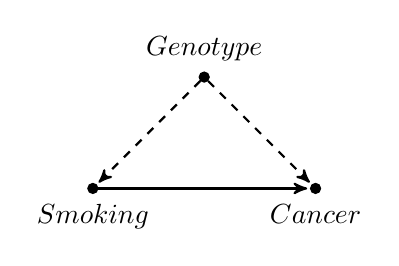
\begin{tikzpicture}[->,>=stealth',shorten >=1pt,auto,node distance=2cm,
  thick,main node/.style={circle,fill=blue!20,draw,font=\sffamily\Large\bfseries}]
               \node (Genotype)  [label = above:$Genotype$,point];
                \node (Smoking) [label = below:$Smoking$ ,below left of = Genotype , point];
                \node (Cancer) [label = below:$Cancer$ ,below right of = Genotype, point];        
                \draw[dashed, ->] (Genotype) -- (Smoking);
                \draw[dashed, ->] (Genotype) -- (Cancer);
                \path (Smoking) edge  (Cancer);
        \end{tikzpicture}
        \caption*{Hopeless}
        \end{figure}
\end{column}
\onslide<4-> 
\begin{column}{.48\textwidth}
\begin{figure}
    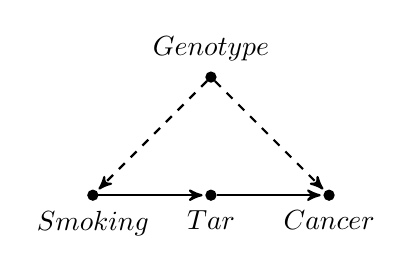
\begin{tikzpicture}[->,>=stealth',shorten >=1pt,auto,node distance=2cm,
  thick,main node/.style={circle,fill=blue!20,draw,font=\sffamily\Large\bfseries}]
               \node at(1.5,1.5) (Genotype)  [label = above:$Genotype$,point];
               \node at(0,0) (Smoking)  [label = below:$Smoking$,point];
               \node at(3,0) (Cancer)  [label = below:$Cancer$,point];
               \node at(1.5,0) (Tar)  [label = below:$Tar$,point];
               \draw[dashed, ->] (Genotype) -- (Smoking);
                \draw[dashed, ->] (Genotype) -- (Cancer);
                \path (Smoking) edge  (Tar);
                \path (Tar) edge  (Cancer);
        \end{tikzpicture}
        \caption*{Solved}
        \end{figure}
\end{column}
\end{columns}
\end{frame}

\begin{frame}{Shut the front door!}
\begin{figure}
    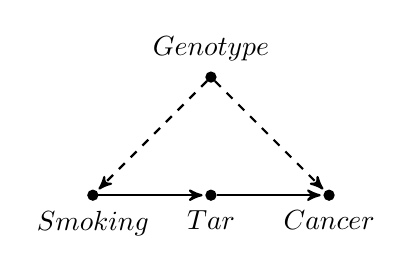
\begin{tikzpicture}[->,>=stealth',shorten >=1pt,auto,node distance=2cm,
  thick,main node/.style={circle,fill=blue!20,draw,font=\sffamily\Large\bfseries}]
               \node at(1.5,1.5) (Genotype)  [label = above:$Genotype$,point];
               \node at(0,0) (Smoking)  [label = below:$Smoking$,point];
               \node at(3,0) (Cancer)  [label = below:$Cancer$,point];
               \node at(1.5,0) (Tar)  [label = below:$Tar$,point];
               \draw[dashed, ->] (Genotype) -- (Smoking);
                \draw[dashed, ->] (Genotype) -- (Cancer);
                \path (Smoking) edge  (Tar);
                \path (Tar) edge  (Cancer);
        \end{tikzpicture}
        \end{figure}
\small
\onslide<1-> Can you ID the effect of smoking on tar? How?\\
\onslide<2-> \[ p(t|do(s)) = p(t|s) \]
\onslide<3-> Can you ID the effect of tar on cancer? How? \\
\onslide<4-> \[p(c|do(t)) = \sum_{S} p(c|t,s)p(s)  \]
\end{frame}

\begin{frame}{Putting the pieces together}
\small
We have:
\begin{itemize}
\item<1-> When tar is set to level $t$,  we see cancer $p(c|do(t))$ of the time.
\item<2-> Smoking causes tar to be at that level as often as often as $p(t|do(s))$
\item<3-> We can combine those into:
\[ p(c|do(s)) = \sum_{t}  p(c|do(t))p(t|do(s)) \]
\item<4-> And we have those pieces:
 \[ p(c|do(s)) = \sum_{t} \sum_{s'} p(C=c|T=t, S=s')  p(S=s')p(T=t| S=s)  \]
\noindent where $s'$ is just an index, to be distinguished from $s$. 
\end{itemize}
\end{frame}
  
%\begin{frame}{Formally now,}
%\small
%\begin{definition}
%\textbf{Front door criterion}.   A set of variables $Z$ is said to satisfy the front-door criterion relative to an ordered pair of variables $(X,Y)$ if
%\footnotesize
%\begin{enumerate}
%\item $Z$ intercepts all directed paths from $X$ to $Y$
%\item There is no unblocked path from $X$ to $Z$
%\item All backdoor paths from $Z$ to $Y$ are blocked by $X$
%\end{enumerate}
%\end{definition}
%\small
%\begin{definition}
%\textbf{Front-door adjustment}. If $Z$ satisfies the front-door criterion relative to $(X,Y)$, and if $P(x,z)>0$, then the causal effect of $X$ on $Y$ is identifiable and is given by the formula
% \[ P(y|do(x)) = \sum_z P(z|x)  \sum_{x'} P(y|x', z) P(x')  \]
%\end{definition}
%\end{frame}

%Brito and Pearl (2002) give a graphical criterion for detecting instrumental variables and instrumental sets in DAGs; and Chan and Kuroki (2010) give graphical criteria for instrument-like auxiliary variable identification strategies.
% Brito, C., & Pearl, J. (2002). Generalized instrumental variables. In A. Darwiche & N. Friedman (Eds.), Uncertainty in artificial intelligence, proceedings of the eighteenth conference(pp. 85–93). San Francisco: Morgan Kaufmann.
%
%Chan, H., & Kuroki, M. (2010). Using descendants as instrumental variables for the identification of direct causal effectsin linear SEMs. In Proceedings of the thirteenth international conference on Artificial Intelligence and Statistics (AISTATS-10) (pp. 73–80), Sardinia, Italy.

\begin{frame}{Are those all the ID strategies DAGs show us?}
\onslide<1-> No. Backdoor and front-door criteria are great tricks, but don't cover every ID strategy justifiable by your graph. \\
\bigskip
\onslide<2-> A \textit{complete} guide is offered by the do-calculus\\
\small
\begin{itemize}
\item Three equalities that you can use (with probability laws) to build any identification result that exists. 
\item Mostly, you know them already, we just need to write them a bit more comprehensively. 
\item It can still take work and creativity to figure out how to apply these rules to get a result, but there is also a algorithm that can find all results
\end{itemize}
\bigskip
\onslide<3-> We won't cover this, but:
\end{frame}
%
%\begin{frame}{Notation}
%\onslide<1-> $G_{\overline{X}}$ is the graph in which you've removed arrows into $X$.
%\small
%\begin{itemize}
%\item Remember: ``parents are above children'', so $\overline{X}$ cuts the lines from parents of $X$ into $X$.
%\item We will use this to establish $do(X)$.
%\end{itemize}
%\normalsize
%\medskip
%\onslide<2-> $G_{\underline{X}}$ is the graph in which you've removed arrows out of $X$
%\begin{itemize}
%\small
%\item You can remember ``parents are below children'', so $\underline{X}$ cuts the lines from $X$ to its children.
%\item This is like the ``trick'' of removing front-door paths that s.t. d-separation implies backdoor criterion.
%%\item If d-separation of Z-Y holds in $G_{\underline{Z}}$, backdoor criterion holds.  (More on this ``trick'' when we discuss CI and graphs). 
%\end{itemize}
%\normalsize
%\medskip
%\onslide<3-> You can combine these, e.g. $G_{\overline{X},\underline{Z}}$
%\end{frame}
%
%\begin{frame}{do-calculus: Rule 1}
%\onslide<1-> You know that
%\begin{itemize}
%\item d-separation s.t. $Y \indep Z | W$ would imply $p(Y|Z, W)=p(Y|W)$.
%\item we usually block an open path containing $W$ by conditioning on $W$, but intervening on $W$ would also block that path.
%\end{itemize}
%\bigskip
%\onslide<2->  All this adds up to a restatement of d-separation:
%\begin{arule}{1. Insertion/deletion of an observation}
%\small
%If $(Y \indep Z | W, X)$ in $G_{\overline{X}}$, then $p(Y | Z, do(x), W) = p(Y | do(x), W)$, 
%\end{arule}
%\end{frame}
%
%%\begin{frame}{Example}
%%
%%\end{frame}
%
%\begin{frame}{do-calculus: Rule 2}
%\small
%\onslide<1-> You know that if $X,W$ satisfies backdoor criterion w.r.t. Z-Y, you can get effect within strata of $X,W$, i.e. $p(Y|do(Z), W)=p(Y|Z,W)$.
%\begin{itemize}
%\item To satisfy, you want to d-separate $Z$ from $Y$, ``but for'' front-door paths
%\item So check d-separation but on $G_{\underline{Z}}$.
%\item Again, you can block paths either by conditioning or intervening. 
%\end{itemize}
%\bigskip
%\onslide<2->  All this adds up to a restatement of the backdoor-criterion:
%\begin{arule}[2. Action/observation exchange]
%$p(y | do(z), do(x), w) = p(y | z, do(x), w)$, if $(Y \indep Z | W, X)$ in $G_{\overline{X}, \underline{Z}}$
%\end{arule}
%\end{frame}
%
%%\begin{frame}{Example}
%%
%%\end{frame}
%
%\begin{frame}{do-calculus: Rule 3}
%\onslide<1-> Blocking paths through $X$ and $W$ (by intervention or conditioning, and while avoiding colliders of $Z$), if $Z$ and $Y$ are independent, $Z$ is not a cause of $Y$.
%\begin{arule}[3. Ignoring actions/interventions]
%$p(y | do(z), do(x), w) = p(y | do(x), w)$, if $(Y \indep Z | W, X)$ in $G_{\overline{X}, \overline{Z(W)}}$
%\end{arule}
%Where $G_{\overline{Z(W)}}$ means you cut arrows into $Z$ except when it is an ancestor of $W$. 
%\begin{itemize}
%\item e.g.  if $G$ is the graph $U \rightarrow Z \rightarrow W \rightarrow Y$, then $G_{\overline{Z(W)}}= G$, since $Z$ is ancestor of $W$.
%\end{itemize}
%\end{frame}
%
%\begin{frame}{In other words:}
%\textbf{Rule 1}:  Detect conditional independence so you can ignore (or add) a conditioning variable.\\
%\bigskip
%\textbf{Rule 2}:  Detect conditional ignorability (via backdoor), so you can replace a $do()$ with ``see'' (or vice versa) \\
%\bigskip
%\textbf{Rule 3}: Detect a non-cause of $Y$, so you can ignore (or add) it.
%\end{frame}
%%\begin{frame}{Example}
%%\end{frame}
%
%\begin{frame}{Front-door via do-calculus}
%\begin{figure}
%    \begin{tikzpicture}[->,>=stealth',shorten >=1pt,auto,node distance=2cm,
%  thick,main node/.style={circle,fill=blue!20,draw,font=\sffamily\Large\bfseries}]
%               \node at(1.5,1.5) (U)  [label = above:$U$,point];
%               \node at(0,0) (X)  [label = below:$X$,point];
%               \node at(3,0) (Y)  [label = below:$Y$,point];
%               \node at(1.5,0) (Z)  [label = below:$Z$,point];
%               \draw[dashed, ->] (U) -- (X);
%                \draw[dashed, ->] (U) -- (Y);
%                \path (X) edge  (Z);
%                \path (Z) edge  (Y);
%        \end{tikzpicture}
%        \caption*{Canonical front-door}
%        \end{figure}
%\small
%It can be tricky to find a path, but two tips: 
%\begin{itemize}
%\item Usually start by writing your query then breaking it up with LIE to see more options. 
%\item We can guess some things the might be useful:
%\begin{itemize}
%\item $p(z|do(x))=p(z|x)$ (rule 2)
%\item $p(y|do(z))$ would be $p(y|z)$ if we blocked $x$ (rule 2)
%\item $do(x)$ won't matter to $Y$ if we've blocked at $z$ (rule 3)
%\end{itemize}
%\end{itemize}
%
%\end{frame}
%
%\begin{frame}{Front-door via do-calculus}
%\small
%\begin{align*}
%p(y|do(x)) &= \sum_z p(y | do(x),z) p(z | do(x)) \quad \text{(LIE)}\\
%&=  \sum_z p(y | z, do(x)) p(z | x) \quad \text{(Rule 2)} \\
%&=  \sum_z p(y | do(z), do(x)) p(z | x) \quad \text{(Rule 2 reverse)} \\
%&=  \sum_z p(y | do(z)) p(z | x) \quad \text{(Rule 3)} \\
%&=  \sum_z \left( \sum_{x'} p(y | do(z), x') p(x'|do(z)) \right) p(z | x) \quad \text{(LIE)} \\
%&=  \sum_z \left( \sum_{x'} p(y | z, x') p(x') \right) p(z | x) \quad \text{(Rules 2,3)}
%% &=  \sum_{z,x'} p(y| x', z)p(z|x)p(x')
%\end{align*}
%
%\end{frame}

\begin{frame}{Causal Fusion -- give it a try}
\begin{center}

\includegraphics[scale=.3]{causalfusion_fd.png}
\end{center}
\end{frame}


\begin{frame}{The identification landscape}
Useful to have this picture in mind:\\
\onslide<2-> \begin{center}

\includegraphics[scale=.5]{IDworld2.png}
\end{center}
\end{frame}


\end{document}
